\documentclass{standalone}

\usepackage[OT1]{fontenc}
\renewcommand*\familydefault{\sfdefault}
\usepackage{helvet,sfmath}
\usepackage{siunitx}

\usepackage{tikz}
\usetikzlibrary{arrows,calc,patterns}
\usepackage{tikz,tkz-euclide}
\usepackage{pgfplots}
\pgfplotsset{compat=1.17}

\begin{document}
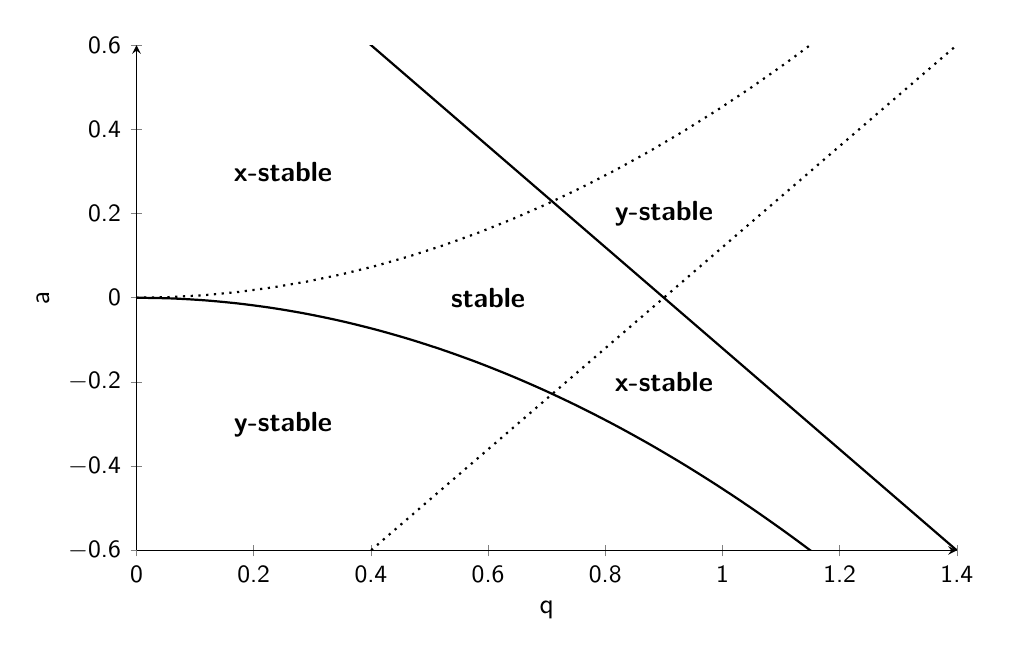
\begin{tikzpicture}
\begin{axis}[
    width=12cm,
    height=8cm,
    xlabel={q},
    ylabel={a},
    xmin=0, xmax=1.4,
    ymin=-0.6, ymax=0.6,
    grid=none,
    axis lines=left,
    xtick={0,0.2,0.4,0.6,0.8,1.0,1.2,1.4},
    ytick={-0.6,-0.4,-0.2,0.0,0.2,0.4,0.6},
    tick label style={font=\small},
    label style={font=\normalsize}
]

\addplot[black, thick, smooth, domain=0:1.4] {-0.4536*x^2};
\addplot[black, dotted, thick, domain=0:1.4] {0.4536*x^2};


% Dotted diagonal lines
\addplot[black, thick, smooth, domain=0:1.4] {-1.2*x+1.08};
\addplot[black, dotted, thick, domain=0:1.4] {1.2*x-1.08};

% Labels for regions
\node at (0.25, 0.3) {\textbf{x-stable}};
\node at (0.25, -0.3) {\textbf{y-stable}};
\node at (0.9, 0.2) {\textbf{y-stable}};
\node at (0.9, -0.2) {\textbf{x-stable}};
\node at (0.6, 0) {\textbf{stable}};

\end{axis}
\end{tikzpicture}
\end{document}